\section{Introduction to Data Flow Analysis}

\subsection{Motivation for Dataflow Analysis}

Some optimizations\footnote{based on \url{https://pages.cs.wisc.edu/~horwitz/CS704-NOTES/2.DATAFLOW.html}} , however, require more "global" information. 
For example, consider the code \ref{lst:expr1}

\begin{lstlisting}[language=C,frame=single, caption=An ,label = lst:expr1]
    a = 1;
    b = 2;
    c = 3;
    if (...) x = a + 5;
    else x = b + 4;
    c = x + 1;
\end{lstlisting}


In this example, the initial assignment to \textit{c} (at line 3) is useless, and the expression 
\textit{x + 1} can be simplified to 7, but it is less obvious how a compiler can discover these facts 
since they cannot be discovered by looking only at one or two consecutive statements. 
A more global analysis is needed so that the compiler knows at each point in the program:
\begin{itemize}
\item    which variables are guaranteed to have constant values, and
\item    which variables will be used before being redefined.
\end{itemize}

To discover these kinds of properties, we use dataflow analysis. 



\subsubsection{What is Data Flow Analysis?}

Local Optimizations only consider optimizations within a node in CFG. 
Data flow analysis will take edges into account, which means composing 
effects of basic blocks to derive information at basic block boundaries.
Data-flow analysis is a technique for gathering information about the possible 
set of values calculated at various points in a computer program. A program's 
control-flow graph (CFG) is used to determine those parts of a program to which 
a particular value assigned to a variable might propagate. The information gathered 
is often used by compilers when optimizing a program. 


Typically, we will do local optimization for the first step to know what happens in a 
basic block, step 2 is to do data flow analysis. In he third step, we will go back and 
revisit the individual instructions inside of the blocks.


Data flow analysis is \textbf{flow-sensitive}, which means we take into account
 the effect of control flow. It is also a \textbf{intraprocedural analysis} which means
 the analysis is within a procedure. Data-flow analysis computes its solutions over the paths in
 a control-flow graph. The well-known, meet-over-all-paths
 formulation produces safe, precise solutions for general dataflow problems. All paths-whether feasible or infeasible,
 heavily or rarely executed-contribute equally to a solution. 

Here are some examples of intraprocedural optimizations:

\begin{itemize}
\item \textbf{constant propagation}. Constant propagation is a well-known global flow analysis 
problem. The goal of constant propagation is to discover values that are constant on all possible 
executions of a program and to propagate these constant values as far forward through the program 
as possible. Expressions whose operands are all constants can be evaluated at compile time and the 
results propagated further.

\item \textbf{common subexpression elimination}

\item \textbf{dead code elimination}. Actually, source code written by programmers doesn't contain
 a lot of dead code, dead code happens to occur partly because of how the front end translates code into 
 the IR. Doing optimizations will also turn code into dead.

\end{itemize}

% \subsection{Static    Program    vs.    Dynamic    Execution }

% Static program 




\subsubsection{Static Program vs. Dynamic Execution}


Program is statically finite, but there can be infinite many dynamic execution paths. On one hand, analysis
 need to be precise, so we will take into account as much dynamic execution as possible. On the other hand, analysis
 need to do the analysis quickly. For a compromise, the analysis result is \textbf{conservative} and what it does is for each 
 point in the program, combines information of all the instances of the same program point.





\subsubsection{Data Flow Analysis Schema}
Before thinking about how to define a dataflow problem, note that there are two kinds of problems:
\begin{itemize}
    \item Forward problems (like constant propagation) where the information at a node n summarizes what can happen on paths from "enter" to n. So if we care about what happened in the past, it's a forward problem.
    \item Backward problems (like live-variable analysis), where the information at a node n summarizes what can happen on paths from n to "exit". So if we care about what will happen in the future, it's a backward problem.
\end{itemize}    

In what follows, we will assume that we're thinking about a forward problem unless otherwise specified.
 
Another way that many common dataflow problems can be categorized is as may problems or must problems. 
The solution to a "may" problem provides information about what may be true at each program point (e.g., 
for live-variables analysis, a variable is considered live after node n if its value may be used before 
being overwritten, while for constant propagation, the pair (x, v) holds before node n if x must have the value v at that point).

Now let's think about how to define a dataflow problem so that it's clear what the (best) solution should be. 
When we do dataflow analysis "by hand", we look at the CFG and think about:

\begin{itemize}
    \item What information holds at the start of the program.
    \item When a node n has more than one incoming edge in the CFG, how to combine the incoming 
    information (i.e., given the information that holds after each predecessor of n, how to 
    combine that information to determine what holds before n).
    \item How the execution of each node changes the information.
\end{itemize}    

This intuition leads to the following definition. An instance of a dataflow problem includes:
\begin{itemize}
    \item a \(CFG\),
    \item a domain \(D\) of "dataflow facts",
    \item a dataflow fact "init" (the information true at the start of the program for forward problems, 
    or at the end of the program for backward problems),
    \item an operator \(\wedge\) (used to combine incoming information from multiple predecessors),
    \item for each CFG node n, a dataflow function \(f_n\) :\( D \rightarrow D\) (that defines the effect of 
    executing n).
\end{itemize} 

For constant propagation, an individual dataflow fact is a set of pairs of the form (var, val),
 so the domain of dataflow facts is the set of all such sets of pairs (the power set). 
 For live-variable analysis, it is the power set of the set of variables in the program.

For both constant propagation and live-variable analysis, the "init" fact is the empty set 
(no variable starts with a constant value, and no variables are live at the end of the program).



For constant propagation, the combining operation \(\wedge\) is set intersection. 
This is because if a node n has two predecessors, p1 and p2, then variable x has value v before 
node n iff it has value v after both p1 and p2. For live-variable analysis, 
\(\wedge\) is set union: if a node n has two successors, s1 and s2, then the value of x after n may be 
used before being overwritten iff that holds either before s1 or before s2. In general, 
for "may" dataflow problems, \(\wedge\) will be some union-like operator, while it will be an intersection-like 
operator for "must" problems.

For constant propagation, the dataflow function associated with a CFG node that does not assign 
to any variable (e.g., a predicate) is the identity function. For a node n that assigns to 
a variable x, there are two possibilities:

\begin{itemize}
\item 1. The right-hand side has a variable that is not constant. In this case, the function 
result is the same as its input except that if variable x was constant the before n, 
it is not constant after n.
\item 2. All right-hand-side variables have constant values. In this case, the right-hand side of 
the assignment is evaluated producing consant-value c, and the dataflow-function result is the 
same as its input except that it includes the pair (x, c) for variable x (and excludes the pair 
for x, if any, that was in the input).
\end{itemize}


For live-variable analysis, the dataflow function for each node n has the form: 
\(f_n(S) = Gen_n \cup (S - KILL_n)\), where \(KILL_n\) is the set of variables defined at node n, 
and \(GEN_n\) is the set of variables used at node n. In other words, for a node that does not 
assign to any variable, the variables that are live before n are those that are live after 
n plus those that are used at n; for a node that assigns to variable x, the variables that are 
live before n are those that are live after n except x, plus those that are used at n 
(including x if it is used at n as well as being defined there).

An equivalent way of formulating the dataflow functions for live-variable analysis is: 
\(f_n(S) = (S \cap NOT-KILL_n) \cup GEN_n\), where \(NOT-KILL_n\) is the set of variables not defined
 at node n. The advantage of this formulation is that it permits the dataflow facts to be 
 represented using bit vectors, and the dataflow functions to be implemented using simple 
 bit-vector operations (and or).

It turns out that a number of interesting dataflow problems have dataflow functions of this 
same form, where \(GEN_n\) and \(KILL_n\) are sets whose definition depends only on n, and the combining 
operator \(\wedge\) is either union or intersection. These problems are called GEN/KILL problems, 
or bit-vector problems.




\subsection{Reaching Definitions}

The Reaching Definitions Problem is a data-flow problem used to answer the
following questions: Which definitions of a variable \textit{X} reach a given use of \textit{X} in
an expression? Is \textit{X} used anywhere before it is defined? A definition\textit{d} reaches a point \textit{p} if there exists path 
from the point immediately following \textit{d} to \textit{p} such that \textit{d} is not killed(overwritten) along that path.



\subsubsection{Iterative   Algorithm}

Here is the iterative  algorithm.



\begin{algorithm}
    \caption{Reaching Defintions:Iterative Algorithm}\label{alg:reachingdefiterative}
    \hspace*{\algorithmicindent} \textbf{Input: control flow graph CFG = (N, E, Entry, Exit) } \\
   
    
    \begin{algorithmic}
   
    \State out[Entry] = $\emptyset$ \algorithmiccomment{Boundary condition}

    \For{\texttt{each basic block B other than Entry}}
        \State \texttt{out[B] = $\emptyset$} \algorithmiccomment{Initialization for iterative algorithm }
    \EndFor
    \While{Changes to any out[] occur}
        \For{\texttt{each basic block B other than Entry}}
        \State \texttt{$in[B] =  \cup (out[p])$, for all predecessors p of B}
        \State \texttt{$out[B] = f_B(in[B])$} \algorithmiccomment{$out[B]=gen[B]\cup (in[B]-kill[B]) $ }
        \EndFor

    \EndWhile
    \end{algorithmic}
\end{algorithm}




\subsubsection{ Worklist   Algorithm}

\begin{algorithm}
    \caption{Reaching Defintions:Worklist Algorithm}\label{alg:reachingdefiterative}
    \hspace*{\algorithmicindent} \textbf{Input: control flow graph CFG = (N, E, Entry, Exit) } \\
   
    
    \begin{algorithmic}
   
    \State out[Entry] = $\emptyset$ \algorithmiccomment{Boundary condition}
    \State \textcolor{blue}{ChangedNodes = N}   
    \For{\texttt{each basic block B other than Entry}}
        \State \texttt{out[B] = $\emptyset$} \algorithmiccomment{Initialization for iterative algorithm }
    \EndFor
    \While{ChangedNodes $\neq \emptyset$}
        \State \textcolor{blue}{Remove i from ChangedNodes}
        \State $in[B] =  \cup (out[p])$, for all predecessors p of B
        \State \textcolor{blue}{$oldout = out[i]$}
        \State $out[i] = f_i(in[i])$ \algorithmiccomment{$out[i]=gen[i]\cup (in[i]-kill[i]) $ }
        \If {\textcolor{blue}{oldout} $\neq out[i]$}

            \For{\texttt{all \textcolor{blue}{successors s of i}}}
                \State \textcolor{blue}{add s to ChangedNodes}
            \EndFor
        \EndIf

    \EndWhile
    \end{algorithmic}
\end{algorithm}



\subsubsection{Example}
Here comes an example of reaching definition.

\begin{figure}[!htb]
    \minipage{0.32\textwidth}
      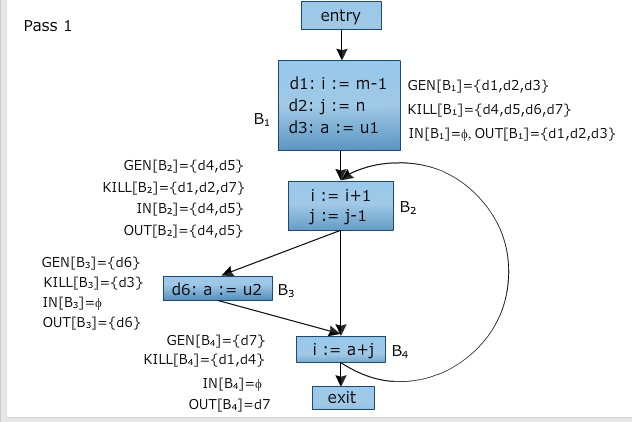
\includegraphics[width=\linewidth]{rdex1.jpg}
      \caption{Pass 1}\label{fig:awesome_image1}
    \endminipage\hfill
    \minipage{0.32\textwidth}
      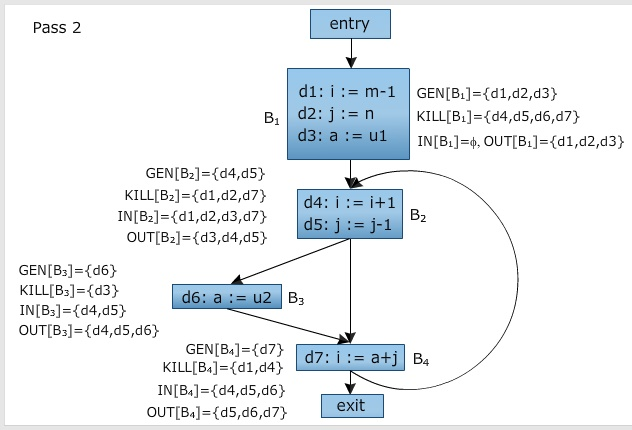
\includegraphics[width=\linewidth]{rdex2.jpg}
      \caption{Pass 2}\label{fig:awesome_image2}
    \endminipage\hfill
    \minipage{0.32\textwidth}%
      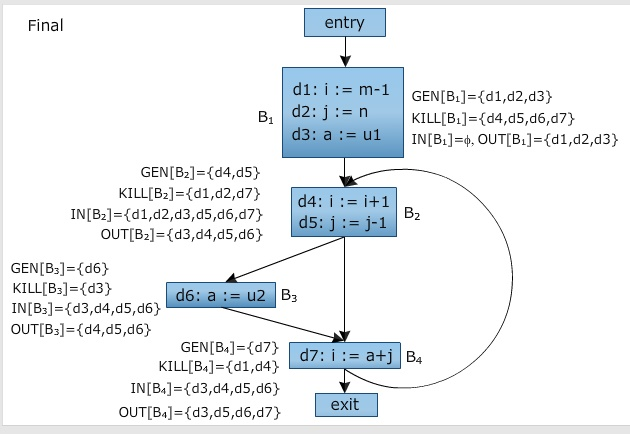
\includegraphics[width=\linewidth]{rdex3.jpg}
      \caption{Pass 3}\label{fig:awesome_image3}
    \endminipage
\end{figure}



\subsection{ Live    Variable    Analysis   }

In compilers, live variable analysis (or simply liveness analysis)
 is a classic data-flow analysis to calculate the variables that 
 are live at each point in the program. A variable is live at 
 some point if it holds a value that may be needed in the future, 
 or equivalently if its value may be read before the next time 
 the variable is written to. \footnote{based on Wikipedia}

\subsubsection{Motivation}

Programs may contain 

\begin{itemize}
\item code which gets executed but which has no useful
effect on the program's overall result;
\item occurrences of variables being used before they
are defined;
\item many variables which need to be allocated
registers and/or memory locations for compilation.

\end{itemize}

The concept of variable liveness is useful in dealing 
with all three of these situations.



\subsubsection{Problem formulation}
Liveness is a data-flow property of variables:
“Is the value of this variable needed?” We therefore 
usually consider liveness from an instruction's 
perspective: each instruction (or node of the
flowgraph) has an associated set of live variables.


\subsubsection{Semantic vs. syntactic\footnote{based on slides from Cambridge University}}


There are two kinds of variable liveness : Semantic liveness and Syntactic liveness.


A variable x is \textbf{semantically} live at a node n if there is
some execution sequence starting at n whose (externally
observable) behaviour can be affected by changing the
value of x. Semantic liveness is concerned with
the execution behaviour of the program.

A variable is \textbf{semantically} live at a node if there is a
path to the exit of the flow graph along which its
value may be used before it is redefined. Syntactic liveness is concerned with properties of
the syntactic structure of the program.


So what is the difference between Semantic liveness and Syntactic liveness? syntactic liveness
is a computable approximation of semantic liveness.


Consider the example 


\begin{lstlisting}[language=C,frame=single, caption=An ,label = lst:expr2]
    int t = x * y;
    if ((x+1)*(x+1) == y) {
     t = 1;
    }
    if (x*x + 2*x + 1 != y) {
     t = 2;
    }
    return t;
\end{lstlisting}

In fact, t is dead in node \texttt{int t = x;} because one of the conditions will be true, 
so on every execution path t is redefined before it is returned.
The value assigned by the first instruction is never used.


But on read path from \ref{fig:liveex} through the
flowgraph, t is not
redefined before it's used,
so t is syntactically live at
the first instruction.Note that this path never
actually occurs during
execution.

\begin{figure}[h]
    \centering
    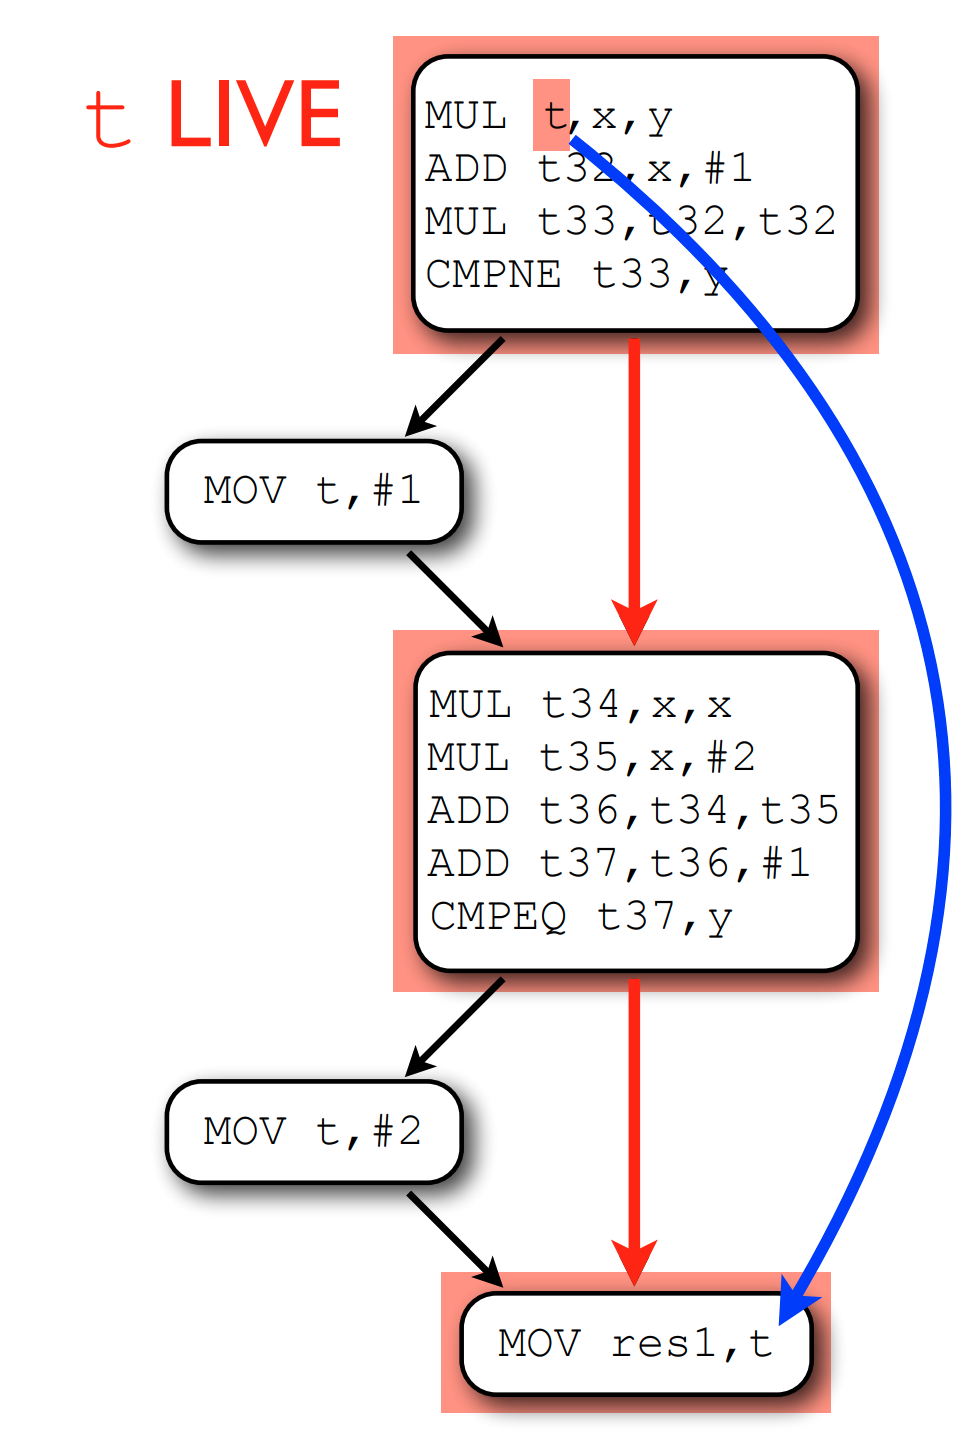
\includegraphics[width=0.3\textwidth]{liveex.png}
    \caption{CFG}
    \label{fig:liveex}
\end{figure}